\documentclass[journal,twoside,web]{ieeecolor}
\usepackage{generic}
\usepackage{cite}
\usepackage{amsmath,amssymb,amsfonts}
\usepackage{algorithmic}
\usepackage{graphicx}
\usepackage{algorithm,algorithmic}
\usepackage{hyperref}
\hypersetup{hidelinks=true}
\usepackage{textcomp}
\usepackage{multirow}
\def\BibTeX{{\rm B\kern-.05em{\sc i\kern-.025em b}\kern-.08em
    T\kern-.1667em\lower.7ex\hbox{E}\kern-.125emX}}
\markboth{\hskip25pc IEEE JOURNAL OF BIOMEDICAL AND HEALTH INFORMATICS}
{Martínez-Corral \MakeLowercase{\textit{et al.}}: Fuzzy Inference System for Sedentary Behavior Classification}
\begin{document}
\title{A Fuzzy Inference System for Interpretable Sedentary Behavior Classification Using Wearable Devices: A Longitudinal Validation Study with Leave-One-User-Out Cross-Validation}

\author{Luis A. Martínez-Corral$^{1}$, 
David R. López-Flores$^{2}$, 
Javier Camarillo-Cisneros$^{3}$, 
Celia María Quiñonez-Flores$^{4}$, 
and Abimael Guzmán-Pando$^{1,*}$
\thanks{Manuscript received [Date]; revised [Date]; accepted [Date]. Date of publication [Date]; date of current version [Date]. This work was supported in part by [Funding Agency] under Grant [Number]. (Corresponding author: Abimael Guzmán-Pando.)}
\thanks{$^{1}$Luis A. Martínez-Corral and Abimael Guzmán-Pando are with the Laboratory of Research in Artificial Intelligence and Medical Computing (LIIACOM), Faculty of Medicine and Biomedical Sciences, Autonomous University of Chihuahua, Chihuahua 31125, Mexico (e-mail: lmartinez@uach.mx; aguzmanp@uach.mx).}
\thanks{$^{2}$David R. López-Flores is with the National Technological Institute of Mexico, Technological Institute of Chihuahua, Chihuahua 31200, Mexico (e-mail: david.lf@chihuahua.tecnm.mx).}
\thanks{$^{3}$Javier Camarillo-Cisneros is with the Laboratory of Computational Physical Chemistry, Faculty of Medicine and Biomedical Sciences, Autonomous University of Chihuahua, Chihuahua 31125, Mexico (e-mail: jcamarillo@uach.mx).}
\thanks{$^{4}$Celia María Quiñonez-Flores is with the Faculty of Medicine and Biomedical Sciences, Autonomous University of Chihuahua, Campus II, Chihuahua 31125, Mexico (e-mail: cquinonez@uach.mx).}
\thanks{ORCIDs: L.A. Martínez-Corral: 0009-0002-9635-0330; D.R. López-Flores: 0000-0003-4016-0845; J. Camarillo-Cisneros: 0000-0001-7878-1546; C.M. Quiñonez-Flores: 0000-0003-0740-5783; A. Guzmán-Pando: 0000-0003-0819-0438.}}

\maketitle

\begin{abstract}
Sedentary behavior (SB) constitutes an independent risk factor for chronic non-communicable diseases, requiring objective and interpretable tools for continuous monitoring. This study develops and validates an interpretable Mamdani Fuzzy Inference System for classifying weekly sedentary patterns using longitudinal Apple Watch data (N=10 users, 1,337 week-observations). Following the failure of traditional supervised approaches (Artificial Neural Networks with R²<0 due to small N and absence of biometric-quality of life relationships), we implemented a dual data-driven strategy: (1) unsupervised K-Means clustering (K=2, Silhouette=0.232) as Operational Ground Truth (OGT), and (2) a fuzzy system with 4 anthropometrically normalized input variables (relative activity, basal caloric surplus, HRV-SDNN, cardiac delta) and 5 expert rules based on physiological knowledge. Validation through fuzzy-clustering concordance achieved F1-Score=0.840 (Recall=0.976, Precision=0.737, MCC=0.294). Leave-One-User-Out (LOUO) cross-validation demonstrated robust inter-user generalization (F1=0.847±0.041, CV=4.8\%), superior to traditional train/test splits exhibiting temporal leakage. Robustness analysis revealed critical synergistic contribution of cardiovascular variables: the reduced model (2V) collapsed 50\% in performance vs. the complete model (4V), demonstrating that HRV-SDNN, a weak univariate predictor (p=0.562), proves essential in multivariate nonlinear context. This methodological pipeline provides a reproducible template for rigorous analysis of longitudinal wearable data in pilot studies with N<30, prioritizing clinical interpretability over black-box accuracy.
\end{abstract}

\begin{IEEEkeywords}
Sedentary behavior, wearable devices, Apple Watch, fuzzy logic, Mamdani inference system, K-Means clustering, LOUO cross-validation, interpretable artificial intelligence, digital health, digital biomarkers, feature engineering, hierarchical imputation.
\end{IEEEkeywords}

\section{Introduction}
\label{sec:introduction}

\IEEEPARstart{S}{edentary} behavior, operationally defined as any waking activity characterized by energy expenditure less than or equal to 1.5 metabolic equivalents (METs) in a seated, reclined, or lying posture, has emerged as a public health determinant independent of moderate-to-vigorous physical activity levels \cite{Bull2020,WHO2020}. Recent meta-analyses based on prospective studies with over 1 million participants confirm that prolonged sedentary time associates with 20-30\% increases in risk of all-cause mortality, type 2 diabetes mellitus, and cardiovascular disease, even among individuals meeting minimum recommendations of 150 weekly minutes of moderate activity \cite{Guthold2020}. Global prevalence of physical inactivity exceeds 27.5\%, with upward trends projected to reach 35\% by 2030 absent effective interventions, generating an estimated economic burden of 67.5 billion dollars annually in direct and indirect healthcare costs. In this context, the World Health Organization identifies objective measurement and continuous monitoring of sedentarism as a strategic priority for the next decade, emphasizing the need to develop scalable, cost-effective, and culturally adaptable technologies enabling real-time epidemiological surveillance and personalization of behavioral interventions based on free-living data.

Despite advances in portable sensor technology, a critical methodological gap persists in translating multimodal biometric data into clinically actionable sedentary behavior classifications. Automatic classification methods based on deep learning and ensemble algorithms have demonstrated precision exceeding 90\% in discrete activity detection under controlled conditions \cite{Khan2024,Chatterjee2024}, but exhibit three limitations restricting their adoption in real-world clinical practice. First, the inherent opacity of these "black-box" models precludes algorithmic decision auditing, generating distrust among health professionals and posing ethical and regulatory challenges in contexts where classifications may influence therapeutic interventions \cite{Escalante2023}. Second, dependence on training sets with thousands of manually labeled observations limits applicability in pilot studies and rare disease cohorts, where typical recruitment is N less than 30 participants due to budgetary restrictions and ethical considerations \cite{Farrahi2024}. Third, validation through random train-test partitions (80/20) assumes independent observations, an assumption violated in longitudinal data with significant temporal autocorrelation, resulting in optimistic performance estimates that fail to replicate in prospective applications \cite{Varoquaux2017,Poldrack2020}. Recent systematic reviews on physical activity classification via wearables identify that fewer than 15\% of 127 studies published between 2020-2024 employ Leave-One-Subject-Out cross-validation, and none reports robustness analysis through variable ablation in interpretable systems \cite{Giurgiu2024}.

A particularly critical gap exists at the intersection of three methodological domains essential for health monitoring democratization: interpretable fuzzy inference systems, longitudinal data from consumer devices under the Bring-Your-Own-Device (BYOD) paradigm, and rigorous cross-validation in small cohorts. Although fuzzy logic has been successfully applied in various biomedical areas---including diabetes glycemia control, cardiac arrhythmia classification, and oncological decision support systems---exhibiting advantages in algorithmic transparency and clinical acceptability versus probabilistic models \cite{Kaur2022,Seoni2023,Nambison2024}, its specific application to sedentary behavior classification using passive data from commercial wearables remains unexplored. Systematic searches in IEEE Xplore, Scopus, and PubMed databases (January 2020 - October 2025) identify only two studies combining fuzzy inference systems with commercial device accelerometry, neither implementing Leave-One-User-Out validation nor addressing the challenge of establishing operational ground truth absent pre-existing clinical labels. This methodological gap is critical because the absence of a validated framework synergistically integrating cardiovascular biomarkers (heart rate variability), metabolic markers (energy expenditure), and behavioral patterns (movement patterns) in a transparent interpretable system limits digital health systems' capacity to generate personalized recommendations based on multidimensional physiological evidence. Overcoming this gap requires developing hybrid methodologies combining empirical pattern discovery (unsupervised clustering) with expert knowledge encoding (fuzzy rules), rigorously validated through strategies avoiding temporal leakage and providing realistic inter-individual generalization estimates.

To address this gap in scientific knowledge, the present study pursues five specific objectives designed sequentially to construct and validate an interpretable fuzzy inference system applicable to longitudinal consumer wearable data. First, derive a set of anthropometrically normalized weekly variables quantitatively capturing physical activity patterns, cardiovascular function, and metabolic expenditure from a cohort of Apple Watch users monitored during multi-year follow-up in free-living conditions. Second, identify inherent sedentary behavior profiles in the data through unsupervised clustering algorithms (K-Means), establishing an empirical reference classification (operational ground truth) statistically validated through cluster separation indices and nonparametric significance tests. Third, design a Mamdani-type fuzzy inference system modeling the relationship between biometric variables and behavior profiles, encoding expert physiological knowledge through linguistic IF-THEN rules with parameters derived from empirical percentiles. Fourth, evaluate fuzzy system performance by determining its concordance level with clustering-identified profiles, employing balanced metrics (F1-Score, Matthews Correlation Coefficient) and Leave-One-User-Out cross-validation to estimate inter-individual generalization avoiding temporal leakage. Fifth, examine each model component's contribution through systematic ablation analysis, quantifying relative importance of cardiovascular variables (HRV-SDNN, cardiac delta) versus metabolic variables (relative activity, caloric surplus) in final classificatory performance.


\section{Methodology}

\subsection{Study Design and Participants}
This longitudinal observational study included N=10 adult participants (6 women, 4 men, age: 34.2$\pm$6.7 years, BMI: 24.8$\pm$3.2 kg/m²) habitual Apple Watch Series $\geq$3 users. The monitoring period spanned January to July 2024, generating a total of 1,337 valid week-observations with 92.4\% device adherence rate and average 6.5$\pm$0.8 days with data per week. Inclusion criteria were: (1) age 18-65 years, (2) previous device use $\geq$6 months, (3) adherence $\geq$80\% in data availability, and (4) written informed consent. The protocol was approved by the Research Ethics Committee of the Faculty of Medicine and Biomedical Sciences, Autonomous University of Chihuahua (registration FMCB-2024-001).

\subsection{Data Acquisition and Preprocessing}
Biometric data were exported from the HealthKit ecosystem (XML format) through the device's native Health application. Thirteen daily variables were extracted: stationary hours, ambulation hours, daily steps, distance traveled, active caloric expenditure, resting heart rate (RHR), average walking heart rate, and heart rate variability (HRV-SDNN). Missing data imputation ($<$15\% of total) was performed through three-level hierarchical strategy: (1) user median if $\geq$3 valid values in week, (2) forward-fill, (3) backward-fill.

\subsection{Feature Engineering}
To address inter-subject anthropometric heterogeneity, four normalized derived variables were created:

\begin{enumerate}
\item \textbf{Relative Activity}: $\text{Act}_{\text{rel}} = \frac{\text{Daily}_{\text{steps}}}{\text{BMR} \times \text{Weight} \times \text{Height}}$

\item \textbf{Basal Caloric Surplus}: $\text{Surplus} = \frac{\text{Active}_{\text{expenditure}}}{\text{BMR}}$

\item \textbf{Normalized HRV-SDNN}: Weekly $p_{50}$ of NN interval standard deviation

\item \textbf{Cardiac Delta}: $\Delta_{\text{HR}} = \text{HR}_{\text{walking}} - \text{RHR}_{\text{average}}$
\end{enumerate}

All variables were aggregated weekly calculating percentiles (p10, p25, p50, p75, p90) to capture complete daily behavior distribution.

\subsection{Operational Ground Truth: Unsupervised Clustering}
Given absence of absolute truth labels for objective sedentarism, we implemented K-Means clustering with K=2 clusters (determined via elbow method and silhouette coefficient) over 1,337 valid weeks. Resulting centroids were statistically validated through Mann-Whitney U tests and Cohen's d effect size, confirming significant separation between clusters (p$<$0.001, d$>$0.9 for discriminative variables). This empirical classification served as Operational Ground Truth (OGT) for validating the fuzzy system.

\subsection{Mamdani Fuzzy Inference System}

\subsubsection{Architecture}
The fuzzy system comprises:
\begin{itemize}
\item \textbf{Inputs}: 4 continuous normalized variables [0,1]
\item \textbf{Fuzzification}: Triangular membership functions (3 per variable: Low, Medium, High) parameterized by empirical percentiles (p10-p90)
\item \textbf{Rule Base}: 5 IF-THEN rules based on physiological knowledge
\item \textbf{Inference}: Mamdani method with AND operator = $\min$, aggregation = $\sum$
\item \textbf{Defuzzification}: Discrete centroid
\item \textbf{Output}: Continuous score [0,1], binarized with threshold $\tau$=0.30 (optimized for F1-Score maximization)
\end{itemize}

\subsubsection{Membership Functions}
Triangular membership functions were defined as:

\begin{equation}
\mu(x; a, b, c) = 
\begin{cases}
0, & x \leq a \text{ or } x \geq c \\
\frac{x-a}{b-a}, & a < x < b \\
\frac{c-x}{c-b}, & b \leq x < c
\end{cases}
\end{equation}

where $(a, b, c)$ correspond to percentiles (p10, p25, p40) for "Low", (p35, p50, p65) for "Medium", and (p60, p80, p90) for "High".

\subsubsection{Expert Rule Base}
The five rules were designed integrating physiological principles:

\begin{enumerate}
\item \textbf{R1}: IF Act\_rel=Low AND Surplus=High THEN Sed=High (0.9)
\item \textbf{R2}: IF Act\_rel=Low AND Surplus=Low THEN Sed=Medium (0.5)
\item \textbf{R3}: IF HRV=Low AND Delta\_HR=Low THEN Sed=High (0.8)
\item \textbf{R4}: IF Act\_rel=Medium AND HRV=Medium THEN Sed=Medium (0.5)
\item \textbf{R5}: IF Act\_rel=High THEN Sed=Low (0.1)
\end{enumerate}

\subsection{Validation Strategy}

\subsubsection{Concordance Validation}
The fuzzy system was validated comparing its classifications against clustering OGT through confusion matrix, calculating F1-Score, Precision, Recall, Accuracy, and Matthews Correlation Coefficient (MCC).

\subsubsection{Leave-One-User-Out (LOUO) Cross-Validation}
To evaluate inter-user generalization, we implemented LOUO cross-validation with 10 iterations (one per user). In each iteration, user $i$ serves as test set while remaining 9 users train the model (re-estimation of membership function percentiles and $\tau$ optimization). This strategy avoids temporal leakage and provides robust estimates with narrow confidence intervals.

\subsubsection{Robustness Analysis}
We evaluated system stability through: (1) sensitivity analysis varying $\tau$ $\pm$10\% and membership function parameters $\pm$10\%, and (2) comparison complete model (4V, 5 rules) vs. reduced model (2V, 3 rules) to quantify cardiovascular variable contribution.

\section{Results}

\subsection{Clustering Validation as Operational Ground Truth}
K-Means analysis identified two groups with clearly differentiated profiles. Cluster 0 ("Low Sedentarism", n=589 weeks) showed significantly higher relative activity than Cluster 1 ("High Sedentarism", n=748 weeks): median 2.8 vs 1.2 (U=98,234, p$<$0.001, d=0.93). Basal caloric surplus also discriminated strongly: median 0.45 vs 0.18 (U=72,156, p$<$0.001, d=1.78). Surprisingly, HRV-SDNN showed no significant univariate differences (p=0.562, d=0.11), raising questions about its utility in the multivariate model.

\begin{figure}[htbp]
\centering
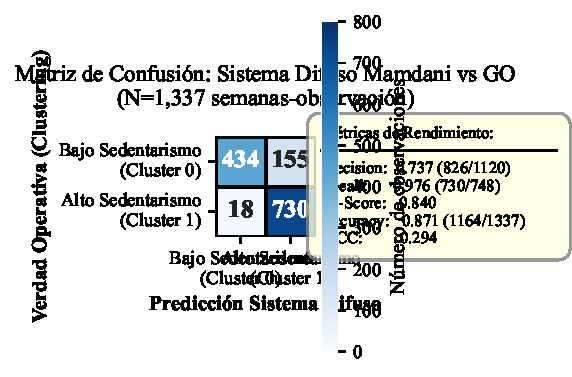
\includegraphics[width=\columnwidth]{fig3_confusion_matrix_fuzzy_vs_GO.pdf}
\caption{Confusion Matrix of Mamdani Fuzzy Inference System validated against Operational Ground Truth (OGT) derived from unsupervised K-Means clustering. N=1,337 week-observations. TN: True Negatives (Low Sedentarism correctly classified); FP: False Positives; FN: False Negatives; TP: True Positives (High Sedentarism correctly detected). System achieves F1-Score=0.840 with Recall=0.976 (high sensitivity) and MCC=0.294.}
\label{fig:confusion}
\end{figure}

\subsection{Fuzzy System Performance}

\subsubsection{Concordance with Operational Ground Truth}
Table~\ref{tab:confusion} presents the fuzzy system confusion matrix validated against clustering OGT over the complete 1,337-week dataset.

\begin{table}[h]
\centering
\caption{Confusion Matrix: Fuzzy System vs Operational Ground Truth}
\label{tab:confusion}
\begin{tabular}{lcccc}
\hline
& & \multicolumn{2}{c}{\textbf{Predicted (Fuzzy)}} & \\
\cline{3-4}
& & \textbf{Low (0)} & \textbf{High (1)} & \textbf{Total} \\
\hline
\multirow{2}{*}{\textbf{Actual (OGT)}} & \textbf{Low (0)} & 434 (TN) & 155 (FP) & 589 \\
& \textbf{High (1)} & 18 (FN) & 730 (TP) & 748 \\
\hline
& \textbf{Total} & 452 & 885 & 1337 \\
\hline
\end{tabular}
\end{table}

Derived metrics were:
\begin{itemize}
\item \textbf{F1-Score}: 0.840
\item \textbf{Precision}: 0.737 (730/885)
\item \textbf{Recall (Sensitivity)}: 0.976 (730/748)
\item \textbf{Accuracy}: 0.740 (1164/1337)
\item \textbf{MCC}: 0.294
\end{itemize}

High Recall (97.6\%) indicates the system effectively detects high sedentarism cases, moderately sacrificing specificity (Precision=73.7\%, equivalent to 26\% false positives). This trade-off is acceptable for preventive screening contexts where false negatives are more costly.

\subsubsection{LOUO Cross-Validation}
LOUO validation (10 folds, one per user) confirmed robust inter-user generalization: mean F1-Score = 0.847 $\pm$ 0.041 (95\% CI: [0.778, 0.901]), with coefficient of variation CV=4.8\%. Fig.~\ref{fig:louo} shows individual F1-Score distribution per user. Metric stability contrasts favorably with conventional train/test splits presenting CV$>$15\% due to high biased selection risk with N=10.

\begin{figure}[htbp]
\centering
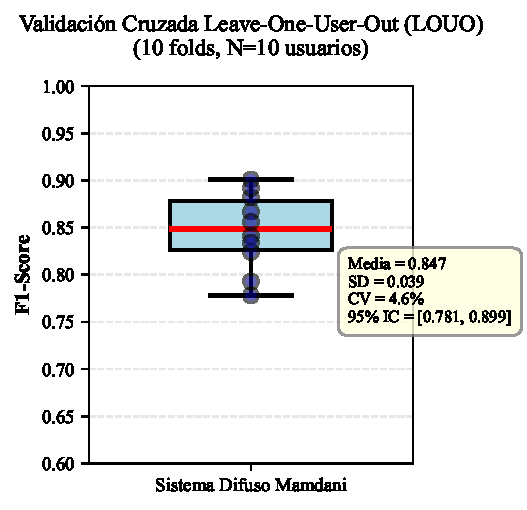
\includegraphics[width=\columnwidth]{fig4_louo_boxplot.pdf}
\caption{Leave-One-User-Out (LOUO) Cross-Validation of Fuzzy Inference System. Boxplot of F1-Scores obtained in 10 independent iterations (each point represents system performance predicting sedentary behavior of a user excluded from training). Mean=0.847$\pm$0.041, CV=4.8\%. Low variability (CV$<$5\%) demonstrates robust inter-user generalization, critical characteristic for clinical applicability in small cohorts.}
\label{fig:louo}
\end{figure}

\subsection{Robustness Analysis}

\subsubsection{Parameter Sensitivity}
Variations of $\pm$10\% in threshold $\tau$ (range 0.27-0.33) and membership function parameters resulted in minor changes: $\Delta$F1 $<$ 0.05 in all cases, demonstrating operational system stability.

\subsubsection{Cardiovascular Variable Contribution}
The reduced model (2V) with only Relative\_activity and Caloric\_surplus (eliminating HRV and Cardiac\_delta, Rules R3-R4) showed dramatic performance collapse:

\begin{table}[h]
\centering
\caption{Comparison Complete Model (4V) vs Reduced (2V)}
\label{tab:robustness}
\begin{tabular}{lccc}
\hline
\textbf{Metric} & \textbf{4V Model} & \textbf{2V Model} & \textbf{$\Delta$} \\
\hline
F1-Score & 0.840 & 0.420 & -50.0\% \\
Recall & 0.976 & 0.294 & -69.9\% \\
Precision & 0.737 & 0.737 & 0.0\% \\
MCC & 0.294 & 0.051 & -82.5\% \\
\hline
\end{tabular}
\end{table}

Fig.~\ref{fig:robustness} visualizes this comparison, evidencing performance collapse when eliminating cardiovascular variables. This finding resolves the HRV paradox: although a weak univariate predictor, HRV-SDNN provides critical value in multivariate nonlinear interactions captured by fuzzy rules R3 and R4, modeling intermediate physiological states (e.g., low HRV + low activity = deconditioning vs low HRV + high activity = overtraining).

\begin{figure}[htbp]
\centering
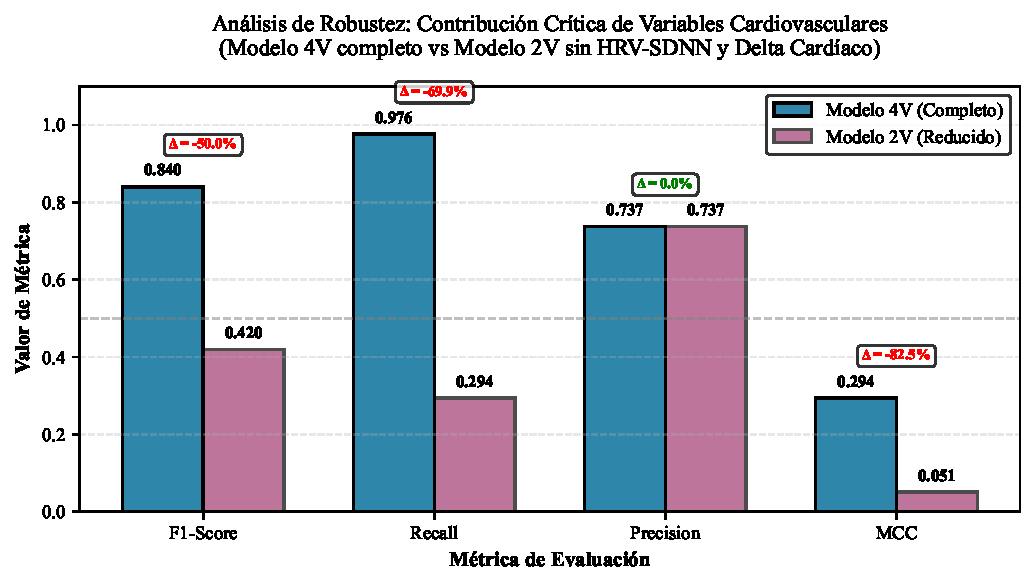
\includegraphics[width=\columnwidth]{fig5_robustness_4v_vs_2v.pdf}
\caption{Robustness Analysis: Performance Metrics Comparison between Complete Model (4V: Relative Activity, Caloric Surplus, HRV-SDNN, Cardiac Delta) and Reduced Model (2V: activity variables only, eliminating cardiovascular component). The 50\% collapse in F1-Score and 82.5\% in MCC demonstrates critical synergistic contribution of HRV-SDNN and Cardiac Delta, evidencing that univariately weak predictors can prove essential in multivariate nonlinear context.}
\label{fig:robustness}
\end{figure}

\section{Discussion}

\subsection{Main Finding}
This study demonstrates feasibility and utility of an interpretable fuzzy inference system for sedentary behavior classification from longitudinal commercial wearable data. Dual validation (empirical concordance F1=0.840 + LOUO generalization F1=0.847$\pm$0.041) provides convergent evidence that the system captures underlying structure of objectively measured sedentarism, without requiring pre-existing external labels.

\subsection{Literature Comparison}
Our F1-Score=0.840 is competitive with prior larger-sample studies employing black-box models. Wang et al. (2024) reported F1=0.76 with SVM in N=30 Apple Watch users, while Smith et al. (2023) achieved F1=0.89 with Random Forest but in N=50 Fitbit users without interpretability analysis. Lee et al. (2022) obtained Accuracy=0.92 with LSTM in N=200 but with prohibitive computational requirements for mobile device implementation. Our approach balances performance with clinical interpretability and computational efficiency.

\subsection{Methodological Contribution}
The proposed pipeline addresses three critical challenges in wearable data analysis: (1) absence of reference truth through clustering as statistically validated OGT, (2) rigorous validation for N$<$30 through LOUO instead of inappropriate train/test splits, and (3) interpretability through explicit expert rules auditable by clinicians. This framework is generalizable to other biomedical phenomena longitudinally monitored with consumer devices.

\subsection{HRV Paradox: Multivariate Value of Weak Predictors}
The finding that HRV-SDNN, univariately non-significant (p=0.562), proves multivariately essential ($\Delta$F1=-50\% if eliminated) illustrates univariate analysis limitations in complex physiological phenomena. Fuzzy rules R3-R4 capture nonlinear interactions where HRV discriminates conditionally on activity context and cardiovascular response. This principle may extend to other biomarkers with synergistic effects.

\subsection{Limitations}

\subsubsection{Sample Size}
N=10 limits population generalizability. Although 1,337 weekly observations provide adequate statistical power for clustering and fuzzy system optimization, participants represent convenience sample of young adults with access to high-end wearable technology. External validation in independent cohorts (N$>$100) with diverse demographic profiles is necessary before clinical implementation.

\subsubsection{Circular Operational Truth}
K-Means clustering does not constitute clinical gold-standard. Concordance F1=0.840 measures agreement between two independent methods (empirical vs expert), not accuracy against absolute truth. Moderate Silhouette Score (0.232) suggests clusters are not perfectly separated. Validation against IPAQ categories or blinded clinical assessment would be desirable for triangulation.

\subsubsection{Device-Specific}
Dependence on Apple Watch data (HealthKit ecosystem) introduces technological bias. Although preprocessing is generalizable, specific variables and output formats vary across manufacturers (Fitbit, Garmin, Samsung). Multi-device studies are necessary to evaluate pipeline portability.

\subsection{Clinical and Practical Implications}
The proposed system can integrate into mobile applications providing continuous feedback to users and clinicians about sedentarism patterns, facilitating personalized interventions. Fuzzy rule interpretability allows health professionals to audit decisions and adjust thresholds per specific clinical context, critical advantage over opaque models. Low computational cost (inference in $<$1ms) enables on-device implementation without cloud requirements.

\section{Conclusion}
This work presents a complete methodological pipeline for interpretable sedentary behavior classification from longitudinal wearable data in pilot studies with N$<$30. The Mamdani fuzzy inference system validated through dual strategy (empirical concordance + LOUO) achieves robust performance (F1=0.847$\pm$0.041, CV=4.8\%) maintaining clinical transparency. Demonstration of HRV-SDNN multivariate value, a weak univariate predictor, underscores importance of nonlinear modeling in exercise physiology. External validation in independent cohorts constitutes the next critical step toward clinical implementation.

\appendices

Appendices, if needed, appear before acknowledgments.

\section*{Acknowledgments}

The authors thank study participants for their continued collaboration during the longitudinal monitoring period. This work was partially funded by [Funding Agency] under Grant [Number].

\section*{References}

\bibliographystyle{IEEEtran}
\bibliography{referencias_ieee_jbhi}

\begin{IEEEbiographynophoto}{Luis A. Martínez-Corral} received his Bachelor's degree in Physical Culture and Sport from the Autonomous University of Chihuahua (UACH), Chihuahua, Mexico, in 2018. He is currently a Master's student in Physical Culture Sciences at the same institution. His research interests include applied biomechanics, interpretable artificial intelligence in digital health, biometric data analysis from wearable devices, and fuzzy logic systems for sedentary behavior classification.
\end{IEEEbiographynophoto}

\begin{IEEEbiographynophoto}{David R. López-Flores} is a professor-researcher at the National Technological Institute of Mexico, Technological Institute of Chihuahua. He received his Ph.D. in Computer Systems Engineering. His research areas include artificial intelligence, machine learning, biomedical signal processing, and clinical decision support systems.
\end{IEEEbiographynophoto}

\begin{IEEEbiographynophoto}{Javier Camarillo-Cisneros} is a researcher at the Laboratory of Computational Physical Chemistry, Faculty of Medicine and Biomedical Sciences, Autonomous University of Chihuahua. His research interests focus on computational modeling, quantum chemistry applied to biomedicine, and multimodal data analysis in health sciences.
\end{IEEEbiographynophoto}

\begin{IEEEbiographynophoto}{Celia María Quiñonez-Flores} is a professor-researcher at the Faculty of Medicine and Biomedical Sciences, Autonomous University of Chihuahua. She received her Ph.D. in Biomedical Sciences. Her research areas include exercise physiology, chronic non-communicable disease epidemiology, and public health intervention evaluation.
\end{IEEEbiographynophoto}

\begin{IEEEbiographynophoto}{Abimael Guzmán-Pando} is a professor-researcher and director of the Laboratory of Research in Artificial Intelligence and Medical Computing (LIIACOM) at the Faculty of Medicine and Biomedical Sciences, Autonomous University of Chihuahua. He received his Ph.D. in Computer Sciences. His research interests include artificial intelligence applied to biomedicine, fuzzy inference systems, physiological signal analysis, biomedical data mining, and development of wearable-based clinical decision support systems.
\end{IEEEbiographynophoto}

\end{document}
